\part{Introduction}
\addto{\captionsenglish}{% Making babel aware of special titles
  \renewcommand{\mtctitle}{Another Title}
}

\startcontents[chapters]
\printmyminitoc{
}


\chapter{Exoplanet detection and characterization using high contrast imaging}
Generally describes what are the advances made in exoplanet detection and characterization
cover those areas where spectra and characterizations are available
\section{Direct exoplanet detections and characterizations}

\chapter{Introduction to machine learning algorithms}
\label{chap:III.2}
Machine learning (ML) algorithms are considered a class of algorithms that learn intrinsic relationships in the data in order to predict specified outputs that depend on these intrinsic relationships in the data.
These relationships between specified outputs and the data can be learned in one of three well known ways,
\begin{enumerate}
    \item \textbf{Unsupervised learning:} where the ML algorithm exploits the intrinsic relationships within data to learn features and use such features to derive the desired output without any external interventions.
    Algorithms in this class are typically used with data where intrinsic relationships in the data are not well established a priory.
    %might be very useful to derive the desired output.
    For example, unsupervised K nearest neighbors algorithms are frequently used to identify clusters within the data that might indicate data grouping which is not easily understood such as looking for data that could be analyzed for transients \citep[e.g][]{2022AleoTransients}, or finding cluster groups in open cluster data \citep[e.g][]{2022cluster}.
    Within Astronomy principal component analysis is a very well known unsupervised ML algorithm typically used in identifying structures in the data that can be discarded.
    Unsupervised ML algorithms are particularly useful for instance in anomaly detection \cite{2023EJASPanomaly}.
    Selecting parameters in the data which will enable other ML algorithms to perform better on the data can also be achieved through unsupervised methods \cite{2023PatRe.14209676H}.
    Principal component analysis is particularly useful in detecting such useful parameters in the data and has been proposed for instance to detect oceans in exoplanet data \citep[e.g][]{2022RyanOCeans}.
    Within the field of high contrast imaging unsupervised ML algorithms have been used in the package \citep[PACO,][]{2023Chomez} and \citep[VIP, ][]{2023Christiaens} also provides this capability. 
    \item \textbf{Supervised learning:} where the algorithm is shown multiple combinations of relationships between desired outputs for a set of inputs over multiple times and thus `trained' to learn the relationship between the input and the output.
    Algorithms in this class are typically used when there is a large amount of labelled data and typically when the relationship between the desired output and input is well known.
    This class of algorithms are also very effective when the desired output represents a non-linear combination of inputs for instance inferring for instance that a picture contains a cat from the presence of whiskers, eyes, nose etc in the picture.
    A famous example of such supervised learning was the handwritten digit recognition where a ML algorithm is trained to recognize handwritten digits in the US postal system and has now been improved on with the latest advances in supervised learning \cite{kussul2004improved}.
    This class comprises of a large set of algorithms spanning from \citep[neural networks,][]{gurney1997introduction} to \citep[random forests,][]{breiman2001random} to modern day \citep[transformers,][]{vaswani2017attention}.
    The advantage of supervised algorithms is that they are able to learn many complex relationships in the data. 
    However, the intrinsic problems of this class is that it requires a large amount of data, where this is relationship is well known.
    Supervised learning schemes suffer from the significant problem of learning the unintended relationships in the data when it is not trained appropriately or it is tested with wrong data.
    In the same example as before, if the algorithm is trained to recognize only cats and we present a dog, it will indeed mis-identify a dog as a cat because of the similarity of the features.
    It is also possible that while learning the possible relationships between the images and the presence of a cat, the algorithm learns that the any indoor setting is a picture of a cat because of our data contained only indoor cats.
    \end{enumerate}
In this thesis, we focused only on supervised learning for the following reasons,
\begin{itemize}
    \item the goal of the my thesis is to derive the presence of an exoplanet given certain discriminatory conditions in my input such as the spectral features corresponding to the planet.
    Such `conditions' are typically called features in ML algorithm training.
    \item a good prior knowledge of such a relationship exists (and is proven using non-ML algorithms such as cross correlation) and a large number of similar datasets exist for me to train a supervised algorithm,
    \item and finally, supervised algorithms allow us to specify the kind of output we need in astrophysics rather than relying on pre-existing relationships within data.
\end{itemize}
The act of producing data pairs of input and desired output is known as `labelling' and is typically carried out before training or testing any algorithms.
The desired outputs which are the result of a specific input combination are respectively called the `label' and the `data'. 
The data, thus, consists of multiple intrinsic parameters which as stated before are called features and the ML algorithm will typically learn which of these features are important for the desired output.
In our case the desired output is whether an extracted spectrum is that of a planet and the features that we use to arrive at this result is the spectral absorption bands.

\section{Types of supervised algorithms}
\label{sec:classifcation and regression}
Supervised learning can be further categorized based on the type of desired output as a regression and classification problems.

\textbf{Regression:} 
When the output of the supervised learning algorithm is a floating point number such as the distance or the intensity then such problems are called regression problems. 
Regression problems are usually adopted when the ML algorithm is meant to produce an unbounded output (except by the intrinsic rules set by the case itself for instance distance cannot be negative). 
This is also useful when we don't know precisely what the expected output is for a specific input, for instance distance between two points in an image can have a infinite values and this changes from each input to another.
Within regression problems, we also have types of regression based on the bounds of the output parameter.
For instance if the bounds are between $0$ and $1$, such regression is known as logistic regression.
The fundamental limitation of the regression problem is that there is an intrinsic uncertainty in the result. 
If sufficient information is presented then this uncertainty can be constrained to be within a few percent.
However, in some cases the output itself is constrained to be within a few finite values. 
Such class of problems are called classification problems.
Astronomy has many regression problems where for example galaxy photometric parameters have been estimated using machine learning algorithms \cite{2022YinAEparameter}.
Time series forecasting in astronomy has also been framed as regression problem \cite{2018Modred}.

\textbf{Classification:}
Classification problems are where the output classes are already well known, for example when the input is a set of words the machine learning algorithms classifies these words in to the emotions they are associated with such as happiness, anger etc. 
Classifiers have been also used to predict for instance liver lesions \cite{2023Nanda} in medical imaging. 
In astronomy classifiers have been used to differentiate between stars, blazars and quasars \cite{2023Zhao} in WISE data.
They have also been famously used to morphologically classify galaxies in the SDSS DR17 \cite{2019MNRASFischer}.
Classifiers in exoplanet direct imaging have been used by \citep[SODINN, ][]{2018Gomez} and \citep[NA-SODINN][]{2023Carlito}.
While classification has the adavantage of knowing the precise set of values that needs to be predicted, it also has the problem of the classes themselves being categorical.
For instance, \citep[SODINN, ][]{2018Gomez} wants the class of $C^{+}$, which is not a numerical value.
Typical classifiers work with either neural networks or ensemble classifiers such as \citep[Random Forests, ][]{breiman2001random} that produce floating point outputs.
In order to convert these numerical values we do the following two step process,
\begin{enumerate}
    \item For an $n$ class classification We first create an $n-1$ sized array.
    Therefore, a $10$ class classifier will output an $9$ element array, 
    \item we then encode the classes using routines such as \citep[One hot encoding][]{harris2010digital} that allows to convert a categorical class into a encoded value, where each position in the array is encoded as a $1$ for its corresponding class.
    The case where all array elements are $0$ also corresponds to a class, thereby covering all classes
\end{enumerate}
This encoded data is now considered as the value that the ML algorithm needs to predict.
Thus the ML algorithm will predict a value for each position in this array, typically values will range between $0$ and $1$ for each position following the sigmoid function.
Each value is thus a probability of the class and thus the class that the algorithm predicts would be the position with the highest probability.
We also at time provide a threshold above which the highest probability is accepted and this becomes the decision boundary of the classifier.

While classifiers are some of the most widely used type of supervised algorithms, they also suffer from the issue where some classes are better represented than the others. 
They also require large number of labelled examples.
These examples have to provide adequate representation of each of the classes, the noise distribution of the noise in each of these class samples should also mimic realistic noise in the data and finally, the samples themselves have to be representative of the data that the algorithm is expected to realistically classify.
In order to meet these requirements, we adopt training methodologies to adequately `train' an algorithm and then adopt specific testing methodologies to realistically estimate the performance of such algorithms. 
These are common for all supervised algorithms, sometimes the testing methodology can still be adopted for unsupervised algorithms as well.
In this thesis when we say ML algorithms it is taken to mean supervised ML algorithms.
\section{Training and testing supervised algorithms}
When generating labels for supervised data there is an intrinsic relationship between the data and its corresponding label.
This relationship could be either linear or non-linear and can thus be mapped to generate the output $y$ from input data $x$ as,
\begin{equation}
    y = f(x)
    \label{eq:y=fx}
\end{equation}
where $f(x)$ represents a function mapping $x$ to $y$
A special case of this linear relationship would be a straight line where $y$ and $x$ are related by its slope $m$ and interecept $c$,
\begin{equation}
    y =  m x + c
    \label{eq:line}
\end{equation}
ML algorithms have been trained in various contexts to derive such relationships between $x$ and $y$ based on large amount of data.
Such a process by which the ML algorithm is tuned to mimic $f(.)$ is called `training'.

Training requires sufficient number of data points that correspond to the expected output $y$. 
The function $f(.)$ is represented by the parameters of the ML algorithm which allow it to produce $y$  given $x$. 
These parameters differ based on the ML algorithm in question, their tuning will be explained in detail in the section corresponding to those class of algorithms.
In order to train an algorithms, we must first prepare the data so that this training is adequate, but not so targeted that the trained `model' can no longer generalize to new data.
The data usually has two characteristic elements, the data or $x$ which consists of images or spectra and the desired result or target output $y$ which is in our case whether the input corresponds to that of a warm Jupiter or not.
In this case it is important that ML algorithm learns the generalized features in the data corresponding to the presence of a warm Jupiter but avoids learning noise structures present only along with the warm Jupiter which would be a systematic of data acquisition.
Typically, this is solved with acquiring data with enough different types of systematics which would convince our model to learn only the common features, since this is not possible to achieve in practise we try to generate large amounts of data and try to evaluate how generalized the model is.
In order to ensure this we first split the data into three parts
\begin{enumerate}
    \item \textbf{Training part}: Usually this comprises of $80\%$ of the data present and is the main engine to train the ML algorithms.
    The training is usually carried out by passing the $x$ through the ML algorithm and `comparing' the output of the algorithm to the true label.
    Usually this comparison is carried out using loss functions such as \citep[cross entropy loss, ][]{1990ZhangCNN}.
    This loss is then minimized over multiple examples by tuning the algorithm until the same error on a part of the dataset not used for training reaches a low minimum value
    \item \textbf{Validation part}: This is the part of the dataset where the loss is tracked until it reaches a low minimum value to signify the end of training. 
    This comprises of $\approx 10\%$ of the total data and is removed from the data before commencing training. 
    The difference between the output produced by passing the validation data through the algorithm and the true labels is not used to tune the ML algorithms but rather serves to mark the state of the algorithm.
    When this difference reaches a minimum low value the training is stopped and the generalization of the algorithm is tested.
    \item \textbf{Testing part:} This part corresponds to $\approx 10\%$ of the total data.
    This part of the data is never passed through the ML algorithm until the error for the validation dataset reaches a low minumum value.
    The test data is treated as the final test data which can be used to benchmark how much the model has generalized. 
    This is also serves to inform if the model has not learnt the features and has just learnt specific noise structures present only in the training data but not present in the test data.
    Note that this does not rule out systematic noise that is present in the entire dataset, and in fact unless the dataset is a very good representation of real variance in data, the results on the test set is usually a clue to the performance of the training.
\end{enumerate}
Thus, the training, validation and test parts make up $100\%$ of the data. 
Typically, when data sizes are small the validation and test are reduced to $5\%$ each.
Once the test part of the data has been passed through the algorithm, the `model' is now deemed as `trained'. 
The quality of the training reflects in the test scores. 
When the test scores are low but the same scores when computed for the training are high, it indicates that the model has not generalized very well.
This is also known as `overfitting'. 
This term refers to the idea that model not only trains on the data features but also on the random noise in the data.
Such a model has to be retrained once again with appropriate mitigation strategies such as regularization in order to avoid such overfitting.
\textbf{Regularization:} is defined as small penalty applied to the error so that the error does not easily minimize for small changes in the data, presumably produced when the model fits the noise.
The converse issue is also possible where the testing error and the training error both are similar but high. 
This is a case of `underfitting' where the data characteristics or features are not sufficiently high to produce a well trained model that generalizes.
In such cases, we have numerous strategies to increase the exposure during training of the algorithm to data features.
\begin{itemize}
    \item \textbf{Feature engineering:} is the strategy where we identify aspects of the data which lead to better validation accuracy and lower training error. 
    We then train the ML algorithm with more of those data samples where such features are present or alternatively train the algorithms with only those features present where we have low validation error.
    \item \textbf{hyperparameter tuning:} in this strategy we change the parameters of the ML algorithm so that it produces lower training error and higher validation accuracy.
    The hyperparameters are subject to which ML algorithm we are training, sometimes tuning such hyperparameters can be difficult to achieve by hand and therefore we undertake a hyperparameter search where we systematically vary the values of the hyperparameters until we achieve the desired accuracy and error combination.
    \item \textbf{data augmentation:} is a method by which we apply specific transforms to the data that systematically provide increased diversity in the features and provide additional noise so that the intrinsic noise is not memorized.
    Thus it also acts as a regularizer.
\end{itemize}

In the subsequent subsection we describe the two broad types of algorithms used in this chapter namely ensemble algorithms of which we will explain the random forests and multi layer perceptrons of which we will describe deep neural networks (DNNs) and autoencoders (AE).
\section{Random forests} 
%Basic idea of ensemble classifiers
Ensemble methods rely on the fundamental idea that an ensemble of methods when polled together produce a reliable and predictive result.
These type of learning methods known as ensemble methods or algorithms was initially proposed with the use of \citep[decision trees, ][]{breiman1998arcing}.
This bit of research was followed by the seminal work where it was shown that \citep[Random forests, ][]{breiman2001random}, which are a collection of decision trees indeed produce smaller test errors than the original decision trees algorithm.
Since then Random forests have been the most sought after algorithm to perform machine learning tasks.
In the field of exoplanets we have instances of the successful use of random forests with \citep[SOFIRF, ][]{2018Gomez} and with \citep[RF, ][]{2020Fisher}.

In this thesis we use the random forest algorithm developed with \citep[scikit-learn, ][]{2011JRFsklearn}.
The basic unit of a random forest is a decision tree.
As the name suggests a decision tree is step by step evaluation of many decisions, which are made based on the data.
Decision trees are frequently used even outside of the ML algorithms to evalaute everyday chocies such as where to eat etc.
A decision tree consists of the following parts:
\begin{itemize}
    \item \textbf{root:} which is the start of the decision tree and is typically the first decision that needs to be made for instance, "Do we want to eat out today?"
    \item\textbf{nodes/leaves:} which is typically a new decision that needs to be made but is only influenced by the previous decision step i.e a node is created when we decide that we do want to eat, however a new decision has to be made about "what food do we want to eat"
    \item \textbf{termination leaf/node:} which is the final decision that is reached and is typically the end of the tree.
\end{itemize}
Depending on how many questions need to be asked and what is the kind of decision that is needed, these trees can be very deep and have many leaves.
A sample tree is show in Fig~\ref{fig:dt}.
This is a typical tree used to evaluate the species of an Iris flower.
This decision tree was expressly chosen indeed for its explanatory value where different characteristics of the Iris flower are used to make choice which finally determine the class such as petal length and width.
\begin{figure}
    \centering
    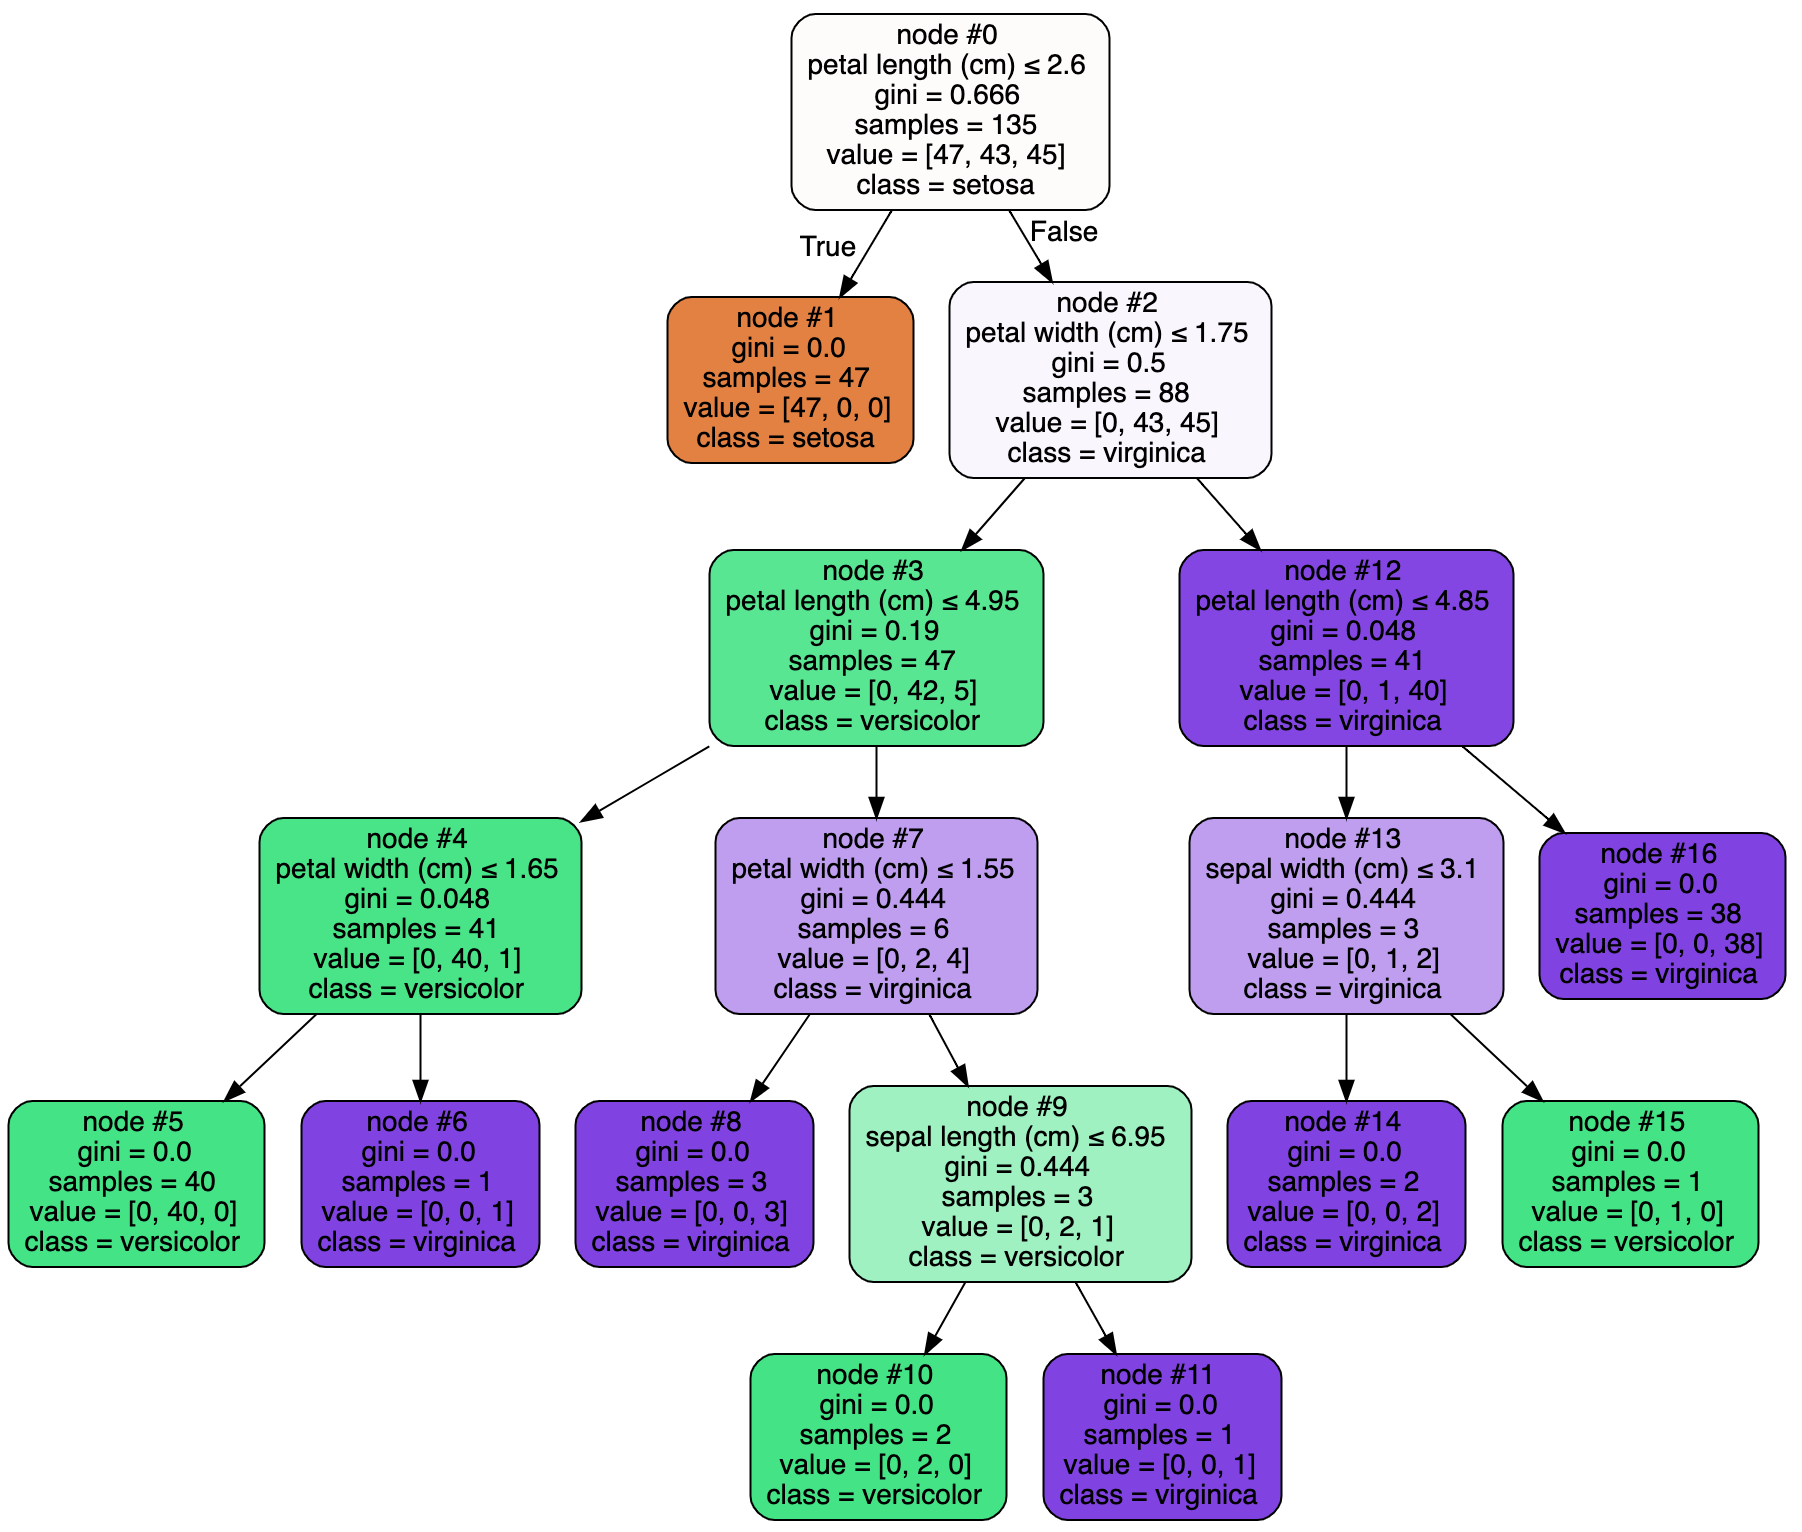
\includegraphics[scale =0.5]{images/Chapter3/decision_tree_model-2609977862.png}
    \caption{A sample decision tree}
    \label{fig:dt}
\end{figure}
An ensemble of many such decision trees result in a `forest' of decision trees which are collectively a `random' forest.

Random forests typically have a number of useful tunable parameters, these parameters are used to both regularize overfitting and improve underfitting.
The most common hyper-parameters that are tuned for random forests are the \texttt{n\_estimators} which are the total number of decision trees in the forest.
A key feature of the random forest is its feature explanability, typically the use of its feature importances, which explain the importance of the different data features in predicting the output of the random forest.
In the example of the Iris species classification, Fig~\ref{fig:RF sample FI} shows the feature importances in predicting the same species as in Fig±\ref{fig:dt}.
The feature importances are relative measures such that the sum of the feature importances is always $1$.
As with the decision tree, the random forest uses multiple features to regress/classify the data and arrive at the desired output.
As it does this process it uses different features, for example in the case of the Iris flower species classification, it uses the petal width as the most important parameter to make this prediction.
This is quite insightful in two ways,
\begin{enumerate}
    \item it is possible to intuit some understanding on the working of the random forest itself by knowing that some features are more relevant to make the desired predictions.
    This is usually the case when we know that the output depends on a few parameters but we are not sure which parameters act as features for the random forest.
    \item it is possible that we have several parameters (as will be the case in my thesis) that could be used to produce the desired output however, we are not sure if this is necessarily true. 
    For example, we have several spectral bins where the absorption lines corresponding to these of an exoplanet are present but we don't know which of these absorption lines allow us to detect and characterize an exoplanet.
\end{enumerate}

Thus, feature importances form the basis to evaluate the features of the data that were learned by the random forest.
This becomes relevant in multiple scenarios, 
\begin{itemize}
    \item when the trained model is overfitting and we can identify and remove those features which produce this overfitting 
    \item when the model is underfitting, the feature importance will allow us to still identify the data features which have a higher relative importance. 
    This can also be problematic because the relative importances can all have very similar values, this is the case when the random forest is not able to fit a generalised model and is the right case for dimensionality reduction
    \item and finally when the model is fitting well and the test and validation accuracies are similar the feature importances are used to study the the features in the data that allow the model to make accurate predictions.
\end{itemize}
\begin{figure}
    \centering
    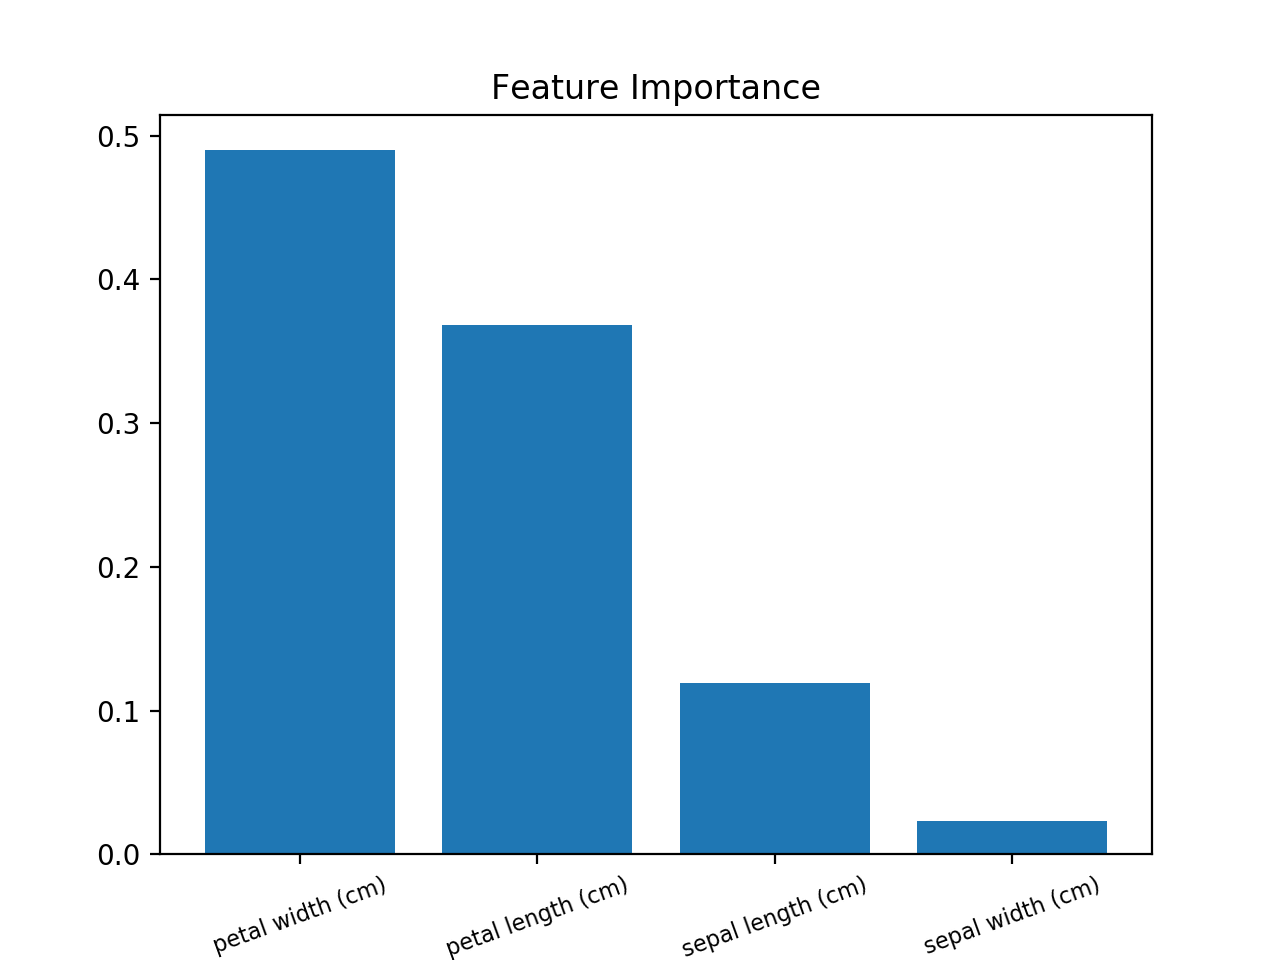
\includegraphics{images/Chapter3/feature_importances_Randomforest.png}
    \caption{RF importances of features used to predict the species of the Iris flower. The y-axis is the relative importance; so a relative importance of $1$ implies the most important and $0$ is the least important feature to predict the species.}
    \label{fig:RF sample FI}
\end{figure}

Random forests are very easily implemented with a two step process with the library \texttt{sklearn} \citep[][]{2011JRFsklearn}.
\section{Multi-layer Perceptrons}
A well known term even amomg non-experts are the words `neural network'.
As the name suggests neural networks are inspired by the network of neurons that make up the mammalian brain.
The basic unit of neural network is a neuron.
A neuron consists of an input, output and an activation function that acts on the input similar to $f(.)$ in Eq~\ref{eq:y=fx}.
This activation function is a mathematical functiom which operates on the input.
Such a unit is called a perceptron and a sample perceptron is depicted in Fig~\ref{fig:perceptron}.
The inputs are combined to form an activation $a_{j}$ via $j$ weights for each input vector value $x_{i}$ making the weight matrix ($w_{ij}$.
The output is defined as ,
\begin{equation}
    y_j = f(\sum_{i=1}^{n} w_{ji}x_i)
    \label{eq: perceptron}
\end{equation}
Many such perceptrons together, producing an output vector $y_{jk}$ for $k$ perceptrons.
This is known as neural network. 
The weights are the neural network parameters whose values can be altered during training.
Activation functions $f(.)$ are typically fixed for the duration of training and varied if the validation results have not reached desirable values.
This is known as a hyper parameter.
The number of neurons in a neural network, the number of weights are also other hyper parameters that can be varied based on the validation results.
The output of a neuron can be treated as an input to another set of perceptrons, and they can be in turn connected to another set of neurons and so on.
Such a network feeds forward the inputs one layer to the next and such networks are called deep neural networks or multi-layer perceptrons.

Based on the kind of combination of $w_{ji}$ and $X_{i}$ perceptron networks can be further sub classified as convolutional neural networks \citep[][]{1990ZhangCNN}, recurrent neural networks and so on.
Neural networks can also work on multi dimensional input as well long vectors.
Configurations of neural networks also vary, for example  other deep neural networks we can also have 

\begin{figure}
    \centering
    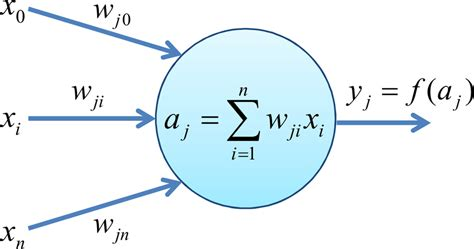
\includegraphics[scale=0.5]{images/Chapter3/perceptron.jpg}
    \caption{A sample percepton consisting of an input vector $X_{i}$ and an output $y$ is depicted here.}
    \label{fig:perceptron}
\end{figure}

\section{Autoencoders}
Autoencoders are special cases of multilayer perceptrons where the input and the output remain fixed but the intermediate layers form a mirrored encoder-decoder structure.
This was first envisioned to denoise data and thus the \citep[denoising autoencoder, ][]{vincent2011connection} was invented.
Typically, the autoencoder has the following main parts,
\begin{itemize}
    \item \textbf{input:} is the input layer which is typically the same shape as the input vector and thus contains as many neurons as the input vector
    \item\textbf{encoder:} the encoder is a set of fully connected neurons which have as input the output of the input layer. 
    These neurons typically are constructed with several layers with the number of neurons in each layer typically reducing in a pyramidal fashion.
    The last layer is the smallest layer and thus the output of this layer is a sparse representation of the input.
    \item\textbf{decoder: } the decoder is a mirror of the encoder both in the layer construction, the number of layers and the neurons used in each layer. 
    It typically terminates in the same number of neurons as the input of the encoder and this layer connects to the output.
    The decoder layer typically reconstructs the input from the sparse representation, thereby recovering a noise free version (note this was the original motivation of the autoencoder).
    \item \textbf{output:} as with the input the output is also a vector equal to the size expected for the output.
\end{itemize}

To wrap this introduction up, we want to make a few points about the limitations of ML algorithms,
\begin{itemize}
    \item \textbf{black box like behavior:} ML algorithms are very useful but also don't particularly lend to great deal of manual fine tuning. 
    Which means that the features that the algorithms learn or not completely controlled and hence to offset this we provide the algorithms with large amount of data.
    \item{\textbf{fine tuning training parameters is challenging:} while there are some thumb rules to follow when training to ensure good training, however there is no way to know if the hyperparameters of the neural network are optimal. 
    Standard techniques such as a parameter space search etc are available but are used when the search itself is not very broad and the parameters have well defined limits}
\end{itemize}
\chapter{Machine learning and astronomy}
\section{Use of deep detection networks}
\section{Applications to exoplanet detection}
\section{Machine learning in direct imaging}
\section{Relevance of using machine learning in simultaneous spectral and imaging targets}
\chapter{Introduction to spectral data processing}\label{chap: II.1}
%Spectral data was used in the previous Part by extracting the spectra from SADI data cubes.
%We used the pixels as samples of spectra that are then cross-correlated with template spectra.
%In order to make detections we had to define a SNR value by using the cross correlations values generated by cross correlating spectra extracted from different pixels.
%In the previous part we explored spectra as extractions from individual pixels.
%We cross correlated these spectra with template spectra and then reconstructed the maps with these replaced spectra.
%We explored different spatial methods to make these spectra noise free and amenable to data processing.
%The goal of the previous part was to understand whether spectral processing of spaxels can produce similar or different effects when taking into account the spectral features.

In this part, we will explore the detectability and characterization of exoplanets through spectra alone without considering the image dimension. 
The goal of this part is to study the detection and characterization of exoplanets whose spectra have been extracted from the spaxels.
In the absence of a spatial dimension, we lack the ability to produce SNR maps as in the previous part, we also miss the distinctive 2D Gaussian shape that indicates the PSF of the telescope on the exoplanet.
Therefore, the broad scientific goal of this part is to understand how much is detectability and characterization of exoplanets is affected by the absence of these key features.
This part will explore the efficacy of ML algorithms of detecting exoplanets and whether they can prove a viable alternative to cross correlation based detection techniques, and whether they can continue to leverage the simultaneous detection and characterization advantage that spectra lend to.

We will describe in this chapter the scientific contributions that spectra alone have produced to the field of exoplanet science, we will then describe briefly the different types of algorithms that have used spectra to make this science possible. 
We will then situate the importance of our research in this context of algorithms by describing the limitations of already present algorithms. 
We will then describe the various ML algorithms that are currently in use in Astronomy related to spectra.
We will then describe why we are motivated to use ML algorithms and which ones seem to be best suited for this job of identifying spectral features in the data.
\section{Exoplanetary spectral data from direct imaging data sets}
As described in the previous part, spectral data are produced using IFS enabled imaging instruments such as \citep[SINFONI, ][]{2004SINFONI} and \citep[GPI, ][]{2014MacintoshGPI}.
The disadvantage of having images with spectra is that it leads to a large number of spectra with just noise and just few spaxels with the exoplanet.
This sometimes leads to false positive detections in discovery campaigns.
In addition, exoplanets are very faint to be easily visible in images, particularly when the image is noisy.
However, it is also possible to not have an explicit spatial dimension, but still have extracted spectra through an IFS enabled instrument.
This allows us to have fewer but more targeted spectra with just one robust noise spectrum, the standard deviation of which can be used to estimate the noise in the observations.
For the purposes of this introductary chapter, we will  refer to such spectra as high contrast diffusion spectra (HDC).

Examples of such instruments include \citep[KPIC, ][]{2019KPIC} and \citep[HARMONI, ]{2022Jocou}.
KPIC is attached to the Keck telescope and is designed to have $\approx 50\%$ starlight suppression and is designed to detect faint exoplanets which are not visible in the image.
Typically, the best way to reduce stellar contamination is to image in wavelength where the stellar flux is low as compared to planetary emissions, the choice of wavelength thus falls typically in the near IR (between $1.4$ $\mu$m  and $1.9$ $\mu$m that corresponds to the H-band and between $2.0$ to $2.4$ $\mu$ m that corresponds to the K- band.
Therefore, these instruments operate in H and/or the K bands.
Typically, KPIC as an example, operates in a domain called high dipsersion coronagraphy which combines high contrast imaging and the medium to high resolution spectroscopy.
The high contrast portion imaging is achieved by feeding the light from the CCD in the telescope through single mode fibers placed at the exact pixel where the planet is present.
The light is then dispersed through medium to high resolution spectrographs with a fixed resolution ($R$) between $10,000-100,000$.
Typically, the $R$ is defined for the lowest wavelength $\lambda_{\rm{min}}$ as,
\begin{equation}
    R =\dfrac{\lambda_{\rm{min}}}{\Delta \lambda}
\end{equation}
where $\Delta \lambda=\lambda_2-\lambda_1$ for consecutive wavelength values $\lambda_2$ and $\lambda_1$.
Laboratory studies have shown, for \citep[e.g][]{2021Calvin}, that coupling the single mode fiber to the CCD pixel appropriately produces the best signal to noise ($\rm{SNR}$).
This $\rm{SNR}$, given the context of using just the spectra defines the `quality' of the spectrum that can be used for scientific processing.

Thus, we have direct imaging that observe a star system where a potential exoplanet is present, the light is gathered on a CCD chip which is then coupled with a single mode fiber to achieve a desired $\rm{SNR}$ and then dispersed through a spectrograph with a fixed $R$ to produce spectra of potential exoplanets.
This spectrum will then be processed similar to what we did in the previous part.
However, unlike in the previous part where we use real data, in this part we will simulate this behaviour without any biases on the efficiency of coupling or the fixed $R$.
In order to achieve this we will use synthetic data that is described in \Cref{chap:III.3}.




\section{Exoplanetary science from HDS}
Spectra from direct imaging instruments have been useful in different ways in the field of exoplanet science. 
Spectra from direct imaging are obtained, usually, through the means integral field spectrographs (IFS) and are typically mounted on larger telescopes that gather photons from the target e.g \citep[e.g][]{2004SINFONI,2019SPHERE} or single mode fiber based instruments such as \citep[e.g][]{2019KPIC}.
This results in gathering of photons in specific wavelength bands that are reflected off the surface of the exoplanet and therefore has the ability to probe interesting surface physics such as temperature, cloud profile etc, when they are appropriately retrieved \citep[e.g][]{2019PICASO}.

There are broadly two ways that these spectra can be used for a) detecting exoplanets based on specific molecules present in the spectrum or b) characterizing exoplanets by identifying the concentration of molecules present in the spectrum.
While detection is a fairly well defined term, meaning to be able to sensitively assert that an exoplanet is present based on spectral features alone, whereas characterization is a broader term that covers a broad swathe of definitions.
The simplest form of characterizing the exoplanet is to constrain the $\rm{T_{eff}}$ and $\log(g)$ of the exoplanet.
In this case the parameters are constrained with a clearly defined error bar for both.
This is usually the first step that follows any detection and spectra are the only data dimension that we have to perform this step.
Usually, we don't need even the spectral absorption lines to estimate $\rm{T_{eff}}$ and $\log(g)$ as shown by \citep[e.g][]{2023Cugno} for PDS70b, they are estimated using continuum modelling or using SED estimation as in the case the first time it was discovered by \cite{2019MesaPDS70}.
Typically, this is the go-to approach when constraining $\rm{T_{eff}}$ and $\log(g)$ is to use the continuum of the exoplanet and derive these with SED, but this only works for exoplanets that are far out from the stellar glare that will be easily characterized.
On the other hand for close in companions such as \citep[HD142527b, ][]{2018A&ChristiaensHD142527}, the continuum is fully dominated by the stellar glow and therefore the molecules present in the atmosphere alone are the indications to the $\rm{T_{eff}}$ and $\log(g)$.

Characterization can also be done in terms of molecular abundances \cite{2023Wangabund} on the surface of the planets, constraining metallicity and surface gravity of the exoplanets \cite{2023AlemanMetall}.
These type of characterizations are particularly interesting because they give us the following scientific details,
\begin{itemize}
    \item \textbf{Constraining the ages of exoplanet systems:} Molecular abundance ratios are crucial in determining how old an exoplanet and thereby its system is which allows us to lay constraints on its theory formation. The \textsc{C/O} ratio is one of the most common ratios that are inferred and \cite{2021Vandermarel} shows that this ratio can be used to constrain the transport rates of icy pebbles within the protoplanetary disks,
    \item \textbf{Constraining the composition of an exoplanet:} the composition of an exoplanet is one of the key attributes that makes exoplanetology truly alluring, according to \cite{2019Madhsudhan} this sort of characterization has resulted in the necessity for new instruments which has in turn lead to a state of `competitive exoplanetology'. Nevertheless, the abundance ratios, the depth at which these ratios are recovered are the only means that we know currently to infer the composition of an exoplanet. 
    \item \textbf{Constraining dynamic processes that define exoplanetary evolution:} molecular species opacities allow astronomers to lay constraints on the dynamic processes within the planetary atmosphere for \citep[e.g Brown dwarfs]{2020Phillips}
    \end{itemize}
In general,characterization using molecular abundances allow us to constrain both the age and rule out potential kinds of exoplanets \citep[e.g][]{2021Christiaens}.

For these kind of studies in addition to observed spectra from planetary systems, we require accurate theoretical models of what planetary spectra look like at different resolutions.
It is prudent to model these spectra in the infra red starting for $0.9$ $\mu$m up to $7$ $\mu$m where the ratio of planetary flux to stellar flux is higher. 
A number of detailed spectral models exist starting with high resolution molecular models produced in lab settings such as ExoMol \cite{2012Tennyson}, detailed atmospheric models that are amenable to spectral retrieval such as PetitRadTrans \cite{2022Molliere}, specialized cloud and atmosphere models that are suited to studying exoplanetary atmospheres such as PICASO3 \cite{2023Mukherjee} and generalized absorption spectra that are more suited to constraining specific properties of the exoplanet such as $\rm{T_{eff}}$ and $\log(\rm{g})$, which is what we use in this project named BT-SETTL \cite{1997Allard}.

While retrieval is notoriously difficult in practice, it is possible to use theoretical spectra and model specific molecules on the surface of the potential exoplanet and thereby characterize them based on mass and temperature.
In order to narrow the scientific scope and to limit the complication of scientific inferences, this thesis will primarily limit itself to characterizing the $\rm{T_{eff}}$ and $\log(g)$.
This also allows this thesis, to explore the effectiveness of the characterization of exoplanets by using the accuracy of characterization of $\rm{T_{eff}}$ and $\log(g)$ as it uses the same features.
These features are also the same molecular absorption lines that will allow us for instance to constrain specific molecular abundances.
Hence, we use these two parameters as proxies to define the ability of an algorithm to characterize exoplanets.
%Such algorithms rely on the accurate modelling of the exoplanet spectra provided by accurate and detailed modelling of the physics necessary to 
%Spectra thus obtained comprise of photons emitted by the star but also the photons reflected off the exoplanet.
\section{Algorithms that detect and/or characterize exoplanets using high contrast diffusion spectra }
%Spectra are particularly useful tools in the infrared where most of the planets are bright as compared to their host stars.
This thesis will constantly refer to algorithms in two broad categories based on how they produce results from the spectra.
These algorithms all either use non-ML based techniques such as cross correlations, forward modelling etc or they use ML based techniques that infer results using ML algorithms that have either been trained with such data or are somehow very specific to using spectra.

Algorithms that use spectra typically work on specific characterizations of a detected exoplanet. 
Atmospheric characterizations are performed by either retrieval algorithms \citep[e.g][]{2017Lavie} or by forward modelling \citep[e.g][]{2023PalmaBifani} the extracted spectra to derive specific atmospheric properties such as carbon to oxygen $\rm{C}$/$\rm{O}$ ratios in the atmosphere of the exoplanet.
Broader characterizations of the exoplanet could be limited to constraining the $\rm{T_{eff}}$ and $\rm{\log(g)}$ with errorbars using log-likelihood ratios obtained through forward modelling \citep[e.g][]{ruffio2019radial} particularly in cases where spectral lines themselves are not well resolved.
In this section, we will discuss algorithms that have one processing criteria in common, they take as input raw spectra from instruments such as KPIC and produce scientifically interpretable and publishable results.
In their turn, these algorithms have been benchmarked for their performance.
In this section we will present a brief summary of the type of algorithms and their science results.

\subsection{Non-ML based spectral inference algorithms }
Post processing for detection and/or characterization of high contrast spectra is different from other spectral post-processing (for example other data acquisition methods such as transit photometry) because of the pecularities unique to high contrast imaging.
The first step, though this thesis does not focus on this step, would be to calibrate the extracted spectra from an instrument.
This calibration step usually involves solving for the wavelength solution so that the resulting vector from the instrument is mapped to its equivalent wavelength values such that each photon value in the vector corresponds to a wavelength vector.
Once this is done, a major problem is the continuous presence of stellar contamination in terms of the stellar continuum in most spectra, particularly those spectra of exoplanets that are at smaller separations from the host star.
Thus, processing of spectra requires the equivalent of the PSF subtraction performed for ADI images.
This has to be followed, by some way of comparing known exoplanet models to the spectrum of the candidate exoplanet in such a way that any residual stellar contamination does not significantly impact this comparison.
Finally, the results of this comparison have to be interpreted so that it has scientific relevance.

\paragraph{Stellar contamination subtraction methods:\\}
The most used stellar contamination subtraction methods is spectral differential imaging \citep[SDI, ][]{2002SparksSDI} which accurately measures the stellar spectrum and subtracts from the data leading to relatively stellar contamination free spectra.
SDI creates several high frequency artefacts which are somewhat resolve with the use of high resolution spectral differential imaging \citep[HRSDI, ][]{2019Haffert} and modified HRSDI \citep[mHRSDI, ][]{2020Xie}.
For spectra in HDS domain, we have continued the same sort reference spectra creation and the adoption of removal of low frequency artifacts.
Usually, this leaves behind mis-subtracted residuals, these are known as speckles in the spatial domain, but there is known equivalent or study in the spectral domain. 
In the spatial domain the speckles are typically tackled using \citep[PCA based algorithms, ][]{2020Xie,2018Hunziker} where after performing procedures such as SDI, further principal components are computed from the image dimension and then subtracted to remove the unsubtracted residuals. 
There has also been a few attempts to combine the advantages of having both image and spectral data by combining angular differential imaging (ADI) and spectral differential imaging techniques in an optimal manner \cite{2021Kiefer}.
This is akin to the analysis we have performed in Part II.
Principal component analysis, typically applied to the image domain \cite{2012Amara}, have been adapted a combination of both spatial and spectral PCA.
%Even then, other than molecular maps, the algorithms do not leverage the information inherently available in spectra to detect exoplanets.
Thus, while we are able to perform basic subtractions there is no comprehensive subtraction of stellar contamination.


\paragraph{modelling the residual spectral features:\\}
Once the stellar contamination subtraction step is completed, algorithms typically now transform the data making it amenable to interpretation and statistical analysis.
There are two broad ways that spectra are processed to characterize them, one would be the so called forward modelling where an analytic function is fit to the data along with a model of noise and the best fit is chosen as the exoplanet model.
An example of such modelling is \citep[BREADS, ][]{2023Agrawal} which uses the standard forward modelling principles set out in \cite{ruffio2019radial} which has been since then in the detection of water and carbon monoxide in HR8799 \citep[][]{2021Ruffio}.
Detailed modeling of the spectral shapes has allowed us to identify orbital parameters as well \cite{2022BWang} where accurate retrieval techniques can be used to constrain the carbon to oxygen ratios as well.
In the realm of medium resolution spectroscopy, it is still possible to limit the science question to if specific molecules such as $\rm{H_2O}$ and $\rm{CO}$ are still detectable and this is performed with radial velocity searches through template cross-correlations \citep[e.g][]{2021Ruffio}.

The other type of processing is using cross correlations of templates and the spectra itself as we did in Part I. 
This type of processing has been particularly popular when detecting specific molecules using \citep[for e.g Molecule maps][]{2018AHoeijmakersMM}. 
Cross correlations have an advantage because of their simplicity and ease of interpretations. 
On the other hand the cross correlation coefficients themselves are noisy and the most consistent interpretations need several noise realizations.
These do not easily lend to HDS data, in this thesis we use the formalism established by \cite{ruffio2019radial} to define cross correlation noise.

\paragraph{interpreting the results:\\}
Both forward modelling and cross correlations result in produces either mock spectral models or cross correlation coefficients that are subject to interpretation.
This interpretation is typically made in the context of statistical $\rm{SNR}$ which is computed as a ratio of the signal cross correlation coefficients and standard deviation of the noise correlations. 
For the forward models the model spectrum is cross correlated with model spectrum produced by the forward model whereas it is also possible for instance to directly cross correlate the spectrum with a template directly.

The $\rm{SNR}$ is then computed for several molecules and thus it is possible to predict if a particular molecule is present if the signal is $5\sigma$ over the noise i.e $\rm{SNR}\ge5$.
Once the presence of an exoplanet molecules are detected, characterization consists of a few more steps in order to derive properties such as abundance ratios, orbital parameters etc.
Typically calculating abundance ratios involves `retrieving' the spectra from a set of atmospheric models as in \citep[for e.g deriving the C/H ratios][]{2022Xuan}.



%It is also possible to turn this question of whether certain molecules exist in the spectra to \textit{where} these molecules exist relative to the host, particularly with direct imaging.
%This kind of analysis is provided by molecular mapping techniques \cite{2018AHoeijmakersMM} where a spatial map is constructed from the cross-correlations of template spectra for each spaxel.
%This has proven particularly useful when trying to detect exoplanets where the planet preferentially radiates in specific wavelengths and is dim in the rest \citep[e.g][]{2019MesaPDS70,2019Haffert}.
%This is usually dependent on the SNR of the extracted spectra themselves.
%Techniques such as molecule mapping \cite{2018AHoeijmakersMM} have been particularly useful to detect exoplanets in specific bands.
%In addition to providing us with such molecule detection maps, spectra also allow us to characterize exoplanetary systems \cite{2018A&ChristiaensHD142527,2019MesaPDS70,2019Haffert} with their constituent molecular species. 
%This is also useful to make a precise atmospheric characterization of exoplanets already detected through other methods \cite{2022Ruffio}.
\subsection{Use of machine learning (ML) algorithms in analyzing astrophysical data and spectra}
Machine learning in the current age of big data has produced algorithms that are capable of analyzing large amounts of data with remarkably small processing times.
They have also proven to be particularly using unsupervised clustering and data mining \citep[e.g][]{2019Baron,2010IBall,2014IVESCI}.
They application of ML algorithms have been particularly of note in classifying stellar spectra \citep[e.g][]{2018Miettinen,2018Naul}.
The analysis of stellar spectra using AstroNN has shown promise even for high resolution spectra \cite{2019Leung}.
Application of artificial neural networks and particularly deep neural networks to exoplanet detection is now regarded as an established method in astrophysics \cite{2020Fluke}.
The exoplanet community has benefited from the use of deep neural networks for Kepler light curves \cite{2018Pearson}, for direct imaging detection \cite{2018Gomez} and to model the PSF model of an instrument \cite{2022Gebhard}.
ML algorithms such as PCA have shown that they can be quite well trusted to model the noise in data \cite{2016A&AGomez} and to model the PSF of the instrument which results in high fidelity subtraction of the stellar components \cite{2014Meshkat}.
In addition, deep learning algorithms such as SODINN \cite{2018Gomez} have demonstrated the ability to detect high contrast companions with fewer false positives.
This has motivated their use in new missions and surveys such as the Large interferometer for exoplanets (LIFE) \cite{2021LIFE}.
In this context, ML algorithms were considered to be of value to the research question that this chapter addresses.
The ML algorithms attempted in direct imaging addresss either the question of PSF subtraction \citep[e.g][]{2022Gebhard} or try to use the spatial noise variance to discriminate between pixels that contain noise and those that contain the exoplanet \citep[e.g]{2018Gomez}.
These methods do not take into account the spectral absorption lines that uniquely identify exoplanetary absorption, which in turn can be considered exoplanetary signatures. 
Some attempts with using spectral features were not particularly successful \citep[e.g][]{2020Fisher} at learning these spectral features unlike \cite{2017RAALi} does for stellar spectra.
However, at this point there still remains the question of why it is necessary to explore the use of ML with spectral data.

\section{Limitations of current methods}
Molecule maps \citep{2018AHoeijmakersMM} are considered suitable for detecting species of molecules of warm Jupiters or cool M-dwarfs \cite{2023Malin} and has been used to further characterize the existence of certain molecules in well known companions \citep[e.g][]{2018Petit}.
One of the greatest limitations with applying techniques such as molecule maps is that they are applied when the existence of an exoplanet is well known and though they lend to astrometric characterization of molecules, it does not allow a truly `blind' search to commence.
In other words, while molecule maps detect the presence of molecules they do not detect the companions themselves, or at any rate they are not designed for a blind search for companions.
In the previous part we redetected HD142527b and produced SNR maps by taking into account all the molecules present in the spectrum.
In the previous part we also demonstrated that it is possible to produce SNR maps of such extracted spaxels and thereby detect a companion and that such a detected companion can also be characterized through the means of characterization matrix that we demonstrated for HD142527b.
Molecule maps and the cross-correlation maps constructed in the previous chapter, rely on some knowledge of spatial noise diversity and the spectral resolution of the spectra play a limited role in detection of the exoplanets.
High resolution spectra can be quite advantageous particularly with forward modeling the spectra \citep[e.g]{2021Ruffio,2021Wang} where spatial data is not available.
However, forward modelling is still a method to \textit{choose} a template that would be cross correlated with the sample exoplanet spectrum.
This brings into focus the importance of the cross correlation as the main engine of comparing spectra and identifying when a template matches the target spectrum.
While there are several algorithms that perform cross correlations and template matching, a unified framework that allows an astronomer to detect and characterize the exoplanet based on the spectrum is still missing.
Existing algorithms are also fine tuned to work with non-ML inference algorithms but a comprehensive study into how amenable these processing steps are with ML algorithms is missing.

Data sizes and the number of spectra available are also on the increase with the advent of James Webb, therefore there needs to be a scalable, accurate and somewhat model independent way to use these high resolution spectra to detect exoplanets in direct imaging.
Computational speeds also are problematic when a large number of forward models need to be run to rule out various hypotheses.
Therefore, the need of the hour is to be able to design an algorithm, which learns specific features which discriminate correctly between the spectra of an exoplanet and those of a star and those of noise.
We also need an algorithm that will be perform similarly for both high and low contrast exoplanets and whose computational complexity does not scale out of bounds for higher resolution spectra.
In this context, ML algorithms are appropriate to be tested with the current suite of inference algorithms already present in the literature.
The question however still remains in terms of why we expect ML algorithms to be effective for this problem.
%We can, therefore, now use spectra with versatility in order to detect and characterize a companion. 
%We also see that ML algorithms are able to detect the presnece of a companion with some degree of astrometric precision.
\section{Motivation to use ML algorithms for identifying spectral features of exoplanets}
%In the previous chapter we have seen that we can use cross-correlation to produce correlation maps which can then be used to produce detection maps.
In the previous part we discovered that detection of exoplanets using spectral data can be done through cross correlation primarily because of the presence of absorption lines in H and K bands.
This was particularly visible when we cross correlated with parts of the spectrum and saw the differential $\rm{SNR}$.
This clearly indicates that data features are not uniform, but are present in different wavelength ranges in the spectrum, this is also the feature set which is utilized for \citep[for e.g ][]{2019Leung} to classify stellar spectra.

However, how effective is an ML algorithm when compared to a standardized cross-correlation algorithm that is described in the previous chapte?
However, is there any relative benefit of using ML algorithms in place of a standard cross correlation and SNR map based detection regime?
Consequently, does this have characterization benefits that is naturally produced by the cross correlations?
What are the ML algorithms that are best suited to this form of analysis and would these `best in class' algorithms provide any advantage to exoplanet detection?
The motivation of this experiment is thus two fold, to begin with we need to define the variables about which we will quantify the effectiveness of an ML algorithm.
The second objective is to verify whether the performance of a well trained ML algorithm offers an advantage to cross-correlation for the same data.

Thus we have organized this part to describe the data that is used to make the comparison, the algorithms used and then finally our conclusion.
This chapter will describe the methods we use to produce data that can be used to test these questions.
We will then describe the control of thse data with the use of parameter `knobs' that allow us to calibrate the effectiveness of the algorithms that we are comparing against.
We will then describe the algorithms that were used during these experiments to compare against the cross correlation of template spectra. 
We will then describe the metrics used to compute the `effectiveness' of an algorithm.
This will the be followed up with describing the results produced by cross correlation and producing thereby the benchmark that is set for the ML algorithms to achieve in order to be called at least `as effective' as ML algorithms.
We will describe these benchmarks for both detection and characterization.
We will then describe results obtained by  cross correlation when the `knobs' are at different levels, for both detection and characterization.
We will then describe the preliminary results for the ML algorithms that will inform us why ML:algorithms cannot be compared with cross correlations.
We will then discuss the reasons for why ML algorithms are not suitable to replace cross correlations in this fashion.
Finally, we will conclude this chapter with a discussion on how we could potentially leverage the power of ML algorithms to improve detectability limits, and leverage what we have learnt from this chapter.